\chapter{Conclusion}\label{chapter:conclusion}
In this work, we have successfully formalised the NP-hardness of 
a few selected classical decision problems.  
The whole work consists of more than 3500 lines of codes, with which we contribute 
six new problems into the Karp21 project. A general overview of the 
progress of the list is given in \hyperref[fig:5.1]{Figure 5.1}.\\\\
The new reductions from this work are linked with red arrows. 
It is also noticed that a reduction from Satisfiability to 3CNF-Satisfiability is not yet
formalised, and should be formalised in the future. With this work,
we manage to show the possibility of formalising and verifying the polynomial-time
reductions and provide a theorectical basis for other works related 
to the complexity theory, especially the NP-hardness. 
\begin{oldfigure}[h!]
\centering 
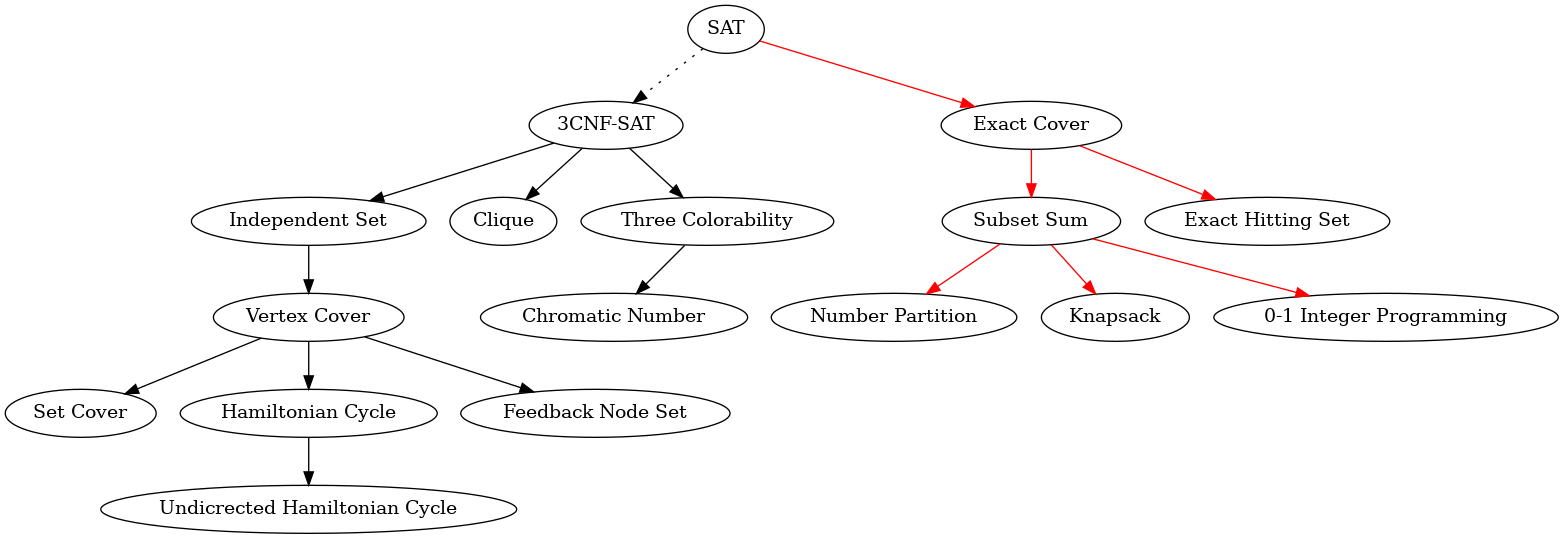
\includegraphics[angle = 90, scale=0.39]{figures/reductions_new.png}
\caption{The updated reduction graph of the Karp21 project.}
\label{fig:5.1}
\end{oldfigure}

\section*{Future Work}
As a future work, it is necessary to add a few more reductions and complete Karp's 
list of twenty-one NP-hard problems. We summarize the remainng problems as follows,
\begin{enumerate}
    \item 3CNF-Satisfiability, Feedback Arc Set, Clique Cover. Reductions to these problems 
    are not related to this work. Reductions are strongly dependent on the previous works.
    \item 3-Dimensional Match, Steiner Tree, Job Sequencing, Max Cut. The reductions 
    presented by Karp are dependent on this work.
\end{enumerate}
Furthermore, a few other classical NP-Hard problems that are not in Karp's list 
can also be added to Karp21 project to make the result more convincing.
Traveling Salesman Problem, for example, 
can be reduced from Hamilton's circuit, while the Bin Packing problem is also 
reducible from Partition. 
